% Options for packages loaded elsewhere
\PassOptionsToPackage{unicode}{hyperref}
\PassOptionsToPackage{hyphens}{url}
\PassOptionsToPackage{dvipsnames,svgnames,x11names}{xcolor}
%
\documentclass[
  ignorenonframetext,
]{beamer}
\usepackage{pgfpages}
\setbeamertemplate{caption}[numbered]
\setbeamertemplate{caption label separator}{: }
\setbeamercolor{caption name}{fg=normal text.fg}
\beamertemplatenavigationsymbolsempty
% Prevent slide breaks in the middle of a paragraph
\widowpenalties 1 10000
\raggedbottom
\setbeamertemplate{part page}{
  \centering
  \begin{beamercolorbox}[sep=16pt,center]{part title}
    \usebeamerfont{part title}\insertpart\par
  \end{beamercolorbox}
}
\setbeamertemplate{section page}{
  \centering
  \begin{beamercolorbox}[sep=12pt,center]{part title}
    \usebeamerfont{section title}\insertsection\par
  \end{beamercolorbox}
}
\setbeamertemplate{subsection page}{
  \centering
  \begin{beamercolorbox}[sep=8pt,center]{part title}
    \usebeamerfont{subsection title}\insertsubsection\par
  \end{beamercolorbox}
}
\AtBeginPart{
  \frame{\partpage}
}
\AtBeginSection{
  \ifbibliography
  \else
    \frame{\sectionpage}
  \fi
}
\AtBeginSubsection{
  \frame{\subsectionpage}
}
\usepackage{amsmath,amssymb}
\usepackage{lmodern}
\usepackage{iftex}
\ifPDFTeX
  \usepackage[T1]{fontenc}
  \usepackage[utf8]{inputenc}
  \usepackage{textcomp} % provide euro and other symbols
\else % if luatex or xetex
  \usepackage{unicode-math}
  \defaultfontfeatures{Scale=MatchLowercase}
  \defaultfontfeatures[\rmfamily]{Ligatures=TeX,Scale=1}
\fi
% Use upquote if available, for straight quotes in verbatim environments
\IfFileExists{upquote.sty}{\usepackage{upquote}}{}
\IfFileExists{microtype.sty}{% use microtype if available
  \usepackage[]{microtype}
  \UseMicrotypeSet[protrusion]{basicmath} % disable protrusion for tt fonts
}{}
\makeatletter
\@ifundefined{KOMAClassName}{% if non-KOMA class
  \IfFileExists{parskip.sty}{%
    \usepackage{parskip}
  }{% else
    \setlength{\parindent}{0pt}
    \setlength{\parskip}{6pt plus 2pt minus 1pt}}
}{% if KOMA class
  \KOMAoptions{parskip=half}}
\makeatother
\usepackage{xcolor}
\newif\ifbibliography
\usepackage{color}
\usepackage{fancyvrb}
\newcommand{\VerbBar}{|}
\newcommand{\VERB}{\Verb[commandchars=\\\{\}]}
\DefineVerbatimEnvironment{Highlighting}{Verbatim}{commandchars=\\\{\}}
% Add ',fontsize=\small' for more characters per line
\usepackage{framed}
\definecolor{shadecolor}{RGB}{248,248,248}
\newenvironment{Shaded}{\begin{snugshade}}{\end{snugshade}}
\newcommand{\AlertTok}[1]{\textcolor[rgb]{0.94,0.16,0.16}{#1}}
\newcommand{\AnnotationTok}[1]{\textcolor[rgb]{0.56,0.35,0.01}{\textbf{\textit{#1}}}}
\newcommand{\AttributeTok}[1]{\textcolor[rgb]{0.77,0.63,0.00}{#1}}
\newcommand{\BaseNTok}[1]{\textcolor[rgb]{0.00,0.00,0.81}{#1}}
\newcommand{\BuiltInTok}[1]{#1}
\newcommand{\CharTok}[1]{\textcolor[rgb]{0.31,0.60,0.02}{#1}}
\newcommand{\CommentTok}[1]{\textcolor[rgb]{0.56,0.35,0.01}{\textit{#1}}}
\newcommand{\CommentVarTok}[1]{\textcolor[rgb]{0.56,0.35,0.01}{\textbf{\textit{#1}}}}
\newcommand{\ConstantTok}[1]{\textcolor[rgb]{0.00,0.00,0.00}{#1}}
\newcommand{\ControlFlowTok}[1]{\textcolor[rgb]{0.13,0.29,0.53}{\textbf{#1}}}
\newcommand{\DataTypeTok}[1]{\textcolor[rgb]{0.13,0.29,0.53}{#1}}
\newcommand{\DecValTok}[1]{\textcolor[rgb]{0.00,0.00,0.81}{#1}}
\newcommand{\DocumentationTok}[1]{\textcolor[rgb]{0.56,0.35,0.01}{\textbf{\textit{#1}}}}
\newcommand{\ErrorTok}[1]{\textcolor[rgb]{0.64,0.00,0.00}{\textbf{#1}}}
\newcommand{\ExtensionTok}[1]{#1}
\newcommand{\FloatTok}[1]{\textcolor[rgb]{0.00,0.00,0.81}{#1}}
\newcommand{\FunctionTok}[1]{\textcolor[rgb]{0.00,0.00,0.00}{#1}}
\newcommand{\ImportTok}[1]{#1}
\newcommand{\InformationTok}[1]{\textcolor[rgb]{0.56,0.35,0.01}{\textbf{\textit{#1}}}}
\newcommand{\KeywordTok}[1]{\textcolor[rgb]{0.13,0.29,0.53}{\textbf{#1}}}
\newcommand{\NormalTok}[1]{#1}
\newcommand{\OperatorTok}[1]{\textcolor[rgb]{0.81,0.36,0.00}{\textbf{#1}}}
\newcommand{\OtherTok}[1]{\textcolor[rgb]{0.56,0.35,0.01}{#1}}
\newcommand{\PreprocessorTok}[1]{\textcolor[rgb]{0.56,0.35,0.01}{\textit{#1}}}
\newcommand{\RegionMarkerTok}[1]{#1}
\newcommand{\SpecialCharTok}[1]{\textcolor[rgb]{0.00,0.00,0.00}{#1}}
\newcommand{\SpecialStringTok}[1]{\textcolor[rgb]{0.31,0.60,0.02}{#1}}
\newcommand{\StringTok}[1]{\textcolor[rgb]{0.31,0.60,0.02}{#1}}
\newcommand{\VariableTok}[1]{\textcolor[rgb]{0.00,0.00,0.00}{#1}}
\newcommand{\VerbatimStringTok}[1]{\textcolor[rgb]{0.31,0.60,0.02}{#1}}
\newcommand{\WarningTok}[1]{\textcolor[rgb]{0.56,0.35,0.01}{\textbf{\textit{#1}}}}
\usepackage{graphicx}
\makeatletter
\def\maxwidth{\ifdim\Gin@nat@width>\linewidth\linewidth\else\Gin@nat@width\fi}
\def\maxheight{\ifdim\Gin@nat@height>\textheight\textheight\else\Gin@nat@height\fi}
\makeatother
% Scale images if necessary, so that they will not overflow the page
% margins by default, and it is still possible to overwrite the defaults
% using explicit options in \includegraphics[width, height, ...]{}
\setkeys{Gin}{width=\maxwidth,height=\maxheight,keepaspectratio}
% Set default figure placement to htbp
\makeatletter
\def\fps@figure{htbp}
\makeatother
\setlength{\emergencystretch}{3em} % prevent overfull lines
\providecommand{\tightlist}{%
  \setlength{\itemsep}{0pt}\setlength{\parskip}{0pt}}
\setcounter{secnumdepth}{-\maxdimen} % remove section numbering
\usepackage{graphicx}
\usepackage{bm}
\definecolor{foreground}{RGB}{255,255,255}
\definecolor{background}{RGB}{34,28,54}
\definecolor{title}{RGB}{105,165,255}
\definecolor{gray}{RGB}{175,175,175}
\definecolor{lightgray}{RGB}{225,225,225}
\definecolor{subtitle}{RGB}{232,234,255}
\definecolor{hilight}{RGB}{112,224,255}
\definecolor{vhilight}{RGB}{255,111,207}
\setbeamertemplate{footline}[page number]
\usepackage{amsthm}
\usepackage{amsmath}
\usepackage{amsfonts}
\usepackage{amscd}
\usepackage{amssymb}
\usepackage{natbib}
\usepackage{url}
\usepackage{tikz}
\ifLuaTeX
  \usepackage{selnolig}  % disable illegal ligatures
\fi
\IfFileExists{bookmark.sty}{\usepackage{bookmark}}{\usepackage{hyperref}}
\IfFileExists{xurl.sty}{\usepackage{xurl}}{} % add URL line breaks if available
\urlstyle{same} % disable monospaced font for URLs
\hypersetup{
  pdftitle={STAT 528 - Advanced Regression Analysis II},
  pdfauthor={Aster models},
  colorlinks=true,
  linkcolor={Maroon},
  filecolor={Maroon},
  citecolor={Blue},
  urlcolor={blue},
  pdfcreator={LaTeX via pandoc}}

\title{STAT 528 - Advanced Regression Analysis II}
\author{Aster models}
\date{}
\institute{Daniel J. Eck\\
Department of Statistics\\
University of Illinois}

\begin{document}
\frame{\titlepage}

\begin{frame}
\newcommand{\R}{\mathbb{R}}
\end{frame}

\begin{frame}{Learning Objectives Today}
\protect\hypertarget{learning-objectives-today}{}
\begin{itemize}
\tightlist
\item
  aster model example
\item
  aster analysis
\end{itemize}
\end{frame}

\begin{frame}{}
\protect\hypertarget{section}{}
The variables under consideration:

\begin{itemize}
\tightlist
\item
  \texttt{nsloc} north-south location of each individual in the
  experimental plot
\item
  \texttt{ewloc} east-west location of each individual in the
  experimental plot
\item
  \texttt{pop} the ancestral population of each individual
\end{itemize}

\vspace{12pt}

Each individual was grown from seed taken from a surviving population in
a prairie remnant in western Minnesota near the Echinacea Project field
site.

Darwinian fitness (our best surrogate of Darwinian fitness) is total
flower head count over the years of data collection.
\end{frame}

\begin{frame}{The aster graph for \emph{Echinacea angustifolia}
(\href{http://echinaceaproject.org/}{aster plants})}
\protect\hypertarget{the-aster-graph-for-aster-plants}{}
\begin{figure}
\begin{tikzpicture}
\put(-100,50){\makebox(0,0){$1$}}
\put(-50,50){\makebox(0,0){$M_1$}}
\put(0,50){\makebox(0,0){$M_2$}}
\put(50,50){\makebox(0,0){$M_3$}}
\put(-87.5,50){\vector(1,0){25}}
\put(-37.5,50){\vector(1,0){25}}
\put(12.5,50){\vector(1,0){25}}
\put(-50,0){\makebox(0,0){$F_1$}}
\put(0,0){\makebox(0,0){$F_2$}}
\put(50,0){\makebox(0,0){$F_3$}}
\put(-50,37.5){\vector(0,-1){25}}
\put(0,37.5){\vector(0,-1){25}}
\put(50,37.5){\vector(0,-1){25}}
\put(-50,-50){\makebox(0,0){$H_1$}}
\put(0,-50){\makebox(0,0){$H_2$}}
\put(50,-50){\makebox(0,0){$H_3$}}
\put(-50,-12.5){\vector(0,-1){25}}
\put(0,-12.5){\vector(0,-1){25}}
\put(50,-12.5){\vector(0,-1){25}}
\end{tikzpicture}
\label{fig:astergraph}
\end{figure}
\end{frame}

\begin{frame}[fragile]{}
\protect\hypertarget{section-1}{}
We load in necessary packages:

\vspace{12pt}

\begin{Shaded}
\begin{Highlighting}[]
\FunctionTok{library}\NormalTok{(tidyverse)}
\FunctionTok{library}\NormalTok{(ggplot2)}
\FunctionTok{library}\NormalTok{(aster)}
\FunctionTok{library}\NormalTok{(aster2)}
\end{Highlighting}
\end{Shaded}
\end{frame}

\begin{frame}[fragile]{Initial data processing}
\protect\hypertarget{initial-data-processing}{}
Here is a brief look at the data:

\vspace{12pt}
\tiny

\begin{Shaded}
\begin{Highlighting}[]
\FunctionTok{data}\NormalTok{(}\StringTok{"echinacea"}\NormalTok{)}
\FunctionTok{names}\NormalTok{(echinacea)}
\end{Highlighting}
\end{Shaded}

\begin{verbatim}
##  [1] "redata"        "repred"        "regroup"       "recode"       
##  [5] "families"      "redelta"       "initial"       "response.name"
##  [9] "pred"          "group"         "code"
\end{verbatim}

\begin{Shaded}
\begin{Highlighting}[]
\FunctionTok{head}\NormalTok{(echinacea}\SpecialCharTok{$}\NormalTok{redata)}
\end{Highlighting}
\end{Shaded}

\begin{verbatim}
##           pop ewloc nsloc varb resp id
## 1.ld02   NWLF    -8   -11 ld02    0  1
## 2.ld02 Eriley    -8   -10 ld02    1  2
## 3.ld02   NWLF    -8    -9 ld02    0  3
## 4.ld02    SPP    -8    -8 ld02    0  4
## 5.ld02    SPP    -8    -7 ld02    0  5
## 6.ld02 Eriley    -8    -6 ld02    1  6
\end{verbatim}
\end{frame}

\begin{frame}[fragile]{}
\protect\hypertarget{section-2}{}
\tiny

\begin{Shaded}
\begin{Highlighting}[]
\NormalTok{echinacea}\SpecialCharTok{$}\NormalTok{redata }\SpecialCharTok{\%\textgreater{}\%} \FunctionTok{filter}\NormalTok{(id }\SpecialCharTok{==} \DecValTok{1}\NormalTok{)}
\end{Highlighting}
\end{Shaded}

\begin{verbatim}
##           pop ewloc nsloc   varb resp id
## 1.ld02   NWLF    -8   -11   ld02    0  1
## 1.ld03   NWLF    -8   -11   ld03    0  1
## 1.ld04   NWLF    -8   -11   ld04    0  1
## 1.fl02   NWLF    -8   -11   fl02    0  1
## 1.fl03   NWLF    -8   -11   fl03    0  1
## 1.fl04   NWLF    -8   -11   fl04    0  1
## 1.hdct02 NWLF    -8   -11 hdct02    0  1
## 1.hdct03 NWLF    -8   -11 hdct03    0  1
## 1.hdct04 NWLF    -8   -11 hdct04    0  1
\end{verbatim}

\begin{Shaded}
\begin{Highlighting}[]
\NormalTok{echinacea}\SpecialCharTok{$}\NormalTok{redata }\SpecialCharTok{\%\textgreater{}\%} \FunctionTok{filter}\NormalTok{(id }\SpecialCharTok{==} \DecValTok{6}\NormalTok{)}
\end{Highlighting}
\end{Shaded}

\begin{verbatim}
##             pop ewloc nsloc   varb resp id
## 6.ld02   Eriley    -8    -6   ld02    1  6
## 6.ld03   Eriley    -8    -6   ld03    1  6
## 6.ld04   Eriley    -8    -6   ld04    1  6
## 6.fl02   Eriley    -8    -6   fl02    0  6
## 6.fl03   Eriley    -8    -6   fl03    0  6
## 6.fl04   Eriley    -8    -6   fl04    1  6
## 6.hdct02 Eriley    -8    -6 hdct02    0  6
## 6.hdct03 Eriley    -8    -6 hdct03    0  6
## 6.hdct04 Eriley    -8    -6 hdct04    1  6
\end{verbatim}
\end{frame}

\begin{frame}[fragile]{}
\protect\hypertarget{section-3}{}
We can see the proportion of individuals that survive each year.

\vspace{12pt}
\tiny

\begin{Shaded}
\begin{Highlighting}[]
\DocumentationTok{\#\# M1}
\NormalTok{echinacea}\SpecialCharTok{$}\NormalTok{redata }\SpecialCharTok{\%\textgreater{}\%} \FunctionTok{filter}\NormalTok{(varb }\SpecialCharTok{==} \StringTok{"ld02"}\NormalTok{) }\SpecialCharTok{\%\textgreater{}\%} \FunctionTok{pull}\NormalTok{(resp) }\SpecialCharTok{\%\textgreater{}\%} \FunctionTok{table}\NormalTok{()}
\end{Highlighting}
\end{Shaded}

\begin{verbatim}
## .
##   0   1 
## 158 412
\end{verbatim}

\begin{Shaded}
\begin{Highlighting}[]
\DocumentationTok{\#\# M2}
\NormalTok{echinacea}\SpecialCharTok{$}\NormalTok{redata }\SpecialCharTok{\%\textgreater{}\%} \FunctionTok{filter}\NormalTok{(id }\SpecialCharTok{\%in\%}\NormalTok{ (echinacea}\SpecialCharTok{$}\NormalTok{redata }\SpecialCharTok{\%\textgreater{}\%} 
                                       \FunctionTok{filter}\NormalTok{(varb }\SpecialCharTok{==} \StringTok{"ld02"} \SpecialCharTok{\&}\NormalTok{ resp }\SpecialCharTok{==} \DecValTok{1}\NormalTok{) }\SpecialCharTok{\%\textgreater{}\%} 
                                       \FunctionTok{pull}\NormalTok{(id)) }\SpecialCharTok{\&}\NormalTok{ varb }\SpecialCharTok{==} \StringTok{"ld03"}\NormalTok{) }\SpecialCharTok{\%\textgreater{}\%} 
  \FunctionTok{pull}\NormalTok{(resp) }\SpecialCharTok{\%\textgreater{}\%} \FunctionTok{table}\NormalTok{()}
\end{Highlighting}
\end{Shaded}

\begin{verbatim}
## .
##   0   1 
##  20 392
\end{verbatim}

\begin{Shaded}
\begin{Highlighting}[]
\DocumentationTok{\#\# M3}
\NormalTok{echinacea}\SpecialCharTok{$}\NormalTok{redata }\SpecialCharTok{\%\textgreater{}\%} \FunctionTok{filter}\NormalTok{(id }\SpecialCharTok{\%in\%}\NormalTok{ (echinacea}\SpecialCharTok{$}\NormalTok{redata }\SpecialCharTok{\%\textgreater{}\%} 
                                       \FunctionTok{filter}\NormalTok{(varb }\SpecialCharTok{==} \StringTok{"ld03"} \SpecialCharTok{\&}\NormalTok{ resp }\SpecialCharTok{==} \DecValTok{1}\NormalTok{) }\SpecialCharTok{\%\textgreater{}\%} 
                                       \FunctionTok{pull}\NormalTok{(id)) }\SpecialCharTok{\&}\NormalTok{ varb }\SpecialCharTok{==} \StringTok{"ld04"}\NormalTok{) }\SpecialCharTok{\%\textgreater{}\%} 
  \FunctionTok{pull}\NormalTok{(resp) }\SpecialCharTok{\%\textgreater{}\%} \FunctionTok{table}\NormalTok{()}
\end{Highlighting}
\end{Shaded}

\begin{verbatim}
## .
##   0   1 
##  14 378
\end{verbatim}
\end{frame}

\begin{frame}[fragile]{}
\protect\hypertarget{section-4}{}
We can see the proportion of individuals that flower each year.

\vspace{12pt}
\tiny

\begin{Shaded}
\begin{Highlighting}[]
\DocumentationTok{\#\# F1}
\NormalTok{echinacea}\SpecialCharTok{$}\NormalTok{redata }\SpecialCharTok{\%\textgreater{}\%} \FunctionTok{filter}\NormalTok{(id }\SpecialCharTok{\%in\%}\NormalTok{ (echinacea}\SpecialCharTok{$}\NormalTok{redata }\SpecialCharTok{\%\textgreater{}\%} 
                                       \FunctionTok{filter}\NormalTok{(varb }\SpecialCharTok{==} \StringTok{"ld02"} \SpecialCharTok{\&}\NormalTok{ resp }\SpecialCharTok{==} \DecValTok{1}\NormalTok{) }\SpecialCharTok{\%\textgreater{}\%} 
                                       \FunctionTok{pull}\NormalTok{(id)) }\SpecialCharTok{\&}\NormalTok{ varb }\SpecialCharTok{==} \StringTok{"fl02"}\NormalTok{) }\SpecialCharTok{\%\textgreater{}\%} 
  \FunctionTok{pull}\NormalTok{(resp) }\SpecialCharTok{\%\textgreater{}\%} \FunctionTok{table}\NormalTok{()}
\end{Highlighting}
\end{Shaded}

\begin{verbatim}
## .
##   0   1 
## 253 159
\end{verbatim}

\begin{Shaded}
\begin{Highlighting}[]
\DocumentationTok{\#\# F2}
\NormalTok{echinacea}\SpecialCharTok{$}\NormalTok{redata }\SpecialCharTok{\%\textgreater{}\%} \FunctionTok{filter}\NormalTok{(id }\SpecialCharTok{\%in\%}\NormalTok{ (echinacea}\SpecialCharTok{$}\NormalTok{redata }\SpecialCharTok{\%\textgreater{}\%} 
                                       \FunctionTok{filter}\NormalTok{(varb }\SpecialCharTok{==} \StringTok{"ld03"} \SpecialCharTok{\&}\NormalTok{ resp }\SpecialCharTok{==} \DecValTok{1}\NormalTok{) }\SpecialCharTok{\%\textgreater{}\%} 
                                       \FunctionTok{pull}\NormalTok{(id)) }\SpecialCharTok{\&}\NormalTok{ varb }\SpecialCharTok{==} \StringTok{"fl03"}\NormalTok{) }\SpecialCharTok{\%\textgreater{}\%} 
  \FunctionTok{pull}\NormalTok{(resp) }\SpecialCharTok{\%\textgreater{}\%} \FunctionTok{table}\NormalTok{()}
\end{Highlighting}
\end{Shaded}

\begin{verbatim}
## .
##   0   1 
## 266 126
\end{verbatim}

\begin{Shaded}
\begin{Highlighting}[]
\DocumentationTok{\#\# F3}
\NormalTok{echinacea}\SpecialCharTok{$}\NormalTok{redata }\SpecialCharTok{\%\textgreater{}\%} \FunctionTok{filter}\NormalTok{(id }\SpecialCharTok{\%in\%}\NormalTok{ (echinacea}\SpecialCharTok{$}\NormalTok{redata }\SpecialCharTok{\%\textgreater{}\%} 
                                       \FunctionTok{filter}\NormalTok{(varb }\SpecialCharTok{==} \StringTok{"ld04"} \SpecialCharTok{\&}\NormalTok{ resp }\SpecialCharTok{==} \DecValTok{1}\NormalTok{) }\SpecialCharTok{\%\textgreater{}\%} 
                                       \FunctionTok{pull}\NormalTok{(id)) }\SpecialCharTok{\&}\NormalTok{ varb }\SpecialCharTok{==} \StringTok{"fl04"}\NormalTok{) }\SpecialCharTok{\%\textgreater{}\%} 
  \FunctionTok{pull}\NormalTok{(resp) }\SpecialCharTok{\%\textgreater{}\%} \FunctionTok{table}\NormalTok{()}
\end{Highlighting}
\end{Shaded}

\begin{verbatim}
## .
##   0   1 
## 162 216
\end{verbatim}
\end{frame}

\begin{frame}[fragile]{}
\protect\hypertarget{section-5}{}
We can see the distribution of head counts each year.

\vspace{12pt}
\tiny

\begin{Shaded}
\begin{Highlighting}[]
\NormalTok{echinacea}\SpecialCharTok{$}\NormalTok{redata }\SpecialCharTok{\%\textgreater{}\%} \FunctionTok{filter}\NormalTok{(id }\SpecialCharTok{\%in\%}\NormalTok{ (echinacea}\SpecialCharTok{$}\NormalTok{redata }\SpecialCharTok{\%\textgreater{}\%} 
                                       \FunctionTok{filter}\NormalTok{(varb }\SpecialCharTok{==} \StringTok{"fl02"} \SpecialCharTok{\&}\NormalTok{ resp }\SpecialCharTok{==} \DecValTok{1}\NormalTok{) }\SpecialCharTok{\%\textgreater{}\%} 
                                       \FunctionTok{pull}\NormalTok{(id)) }\SpecialCharTok{\&}\NormalTok{ varb }\SpecialCharTok{==} \StringTok{"hdct02"}\NormalTok{) }\SpecialCharTok{\%\textgreater{}\%} 
  \FunctionTok{pull}\NormalTok{(resp) }\SpecialCharTok{\%\textgreater{}\%} \FunctionTok{hist}\NormalTok{(., }\AttributeTok{main =} \StringTok{"Distribution of hdct02"}\NormalTok{)}
\end{Highlighting}
\end{Shaded}

\includegraphics{week14p2_files/figure-beamer/unnamed-chunk-6-1.pdf}
\end{frame}

\begin{frame}[fragile]{}
\protect\hypertarget{section-6}{}
\tiny

\begin{Shaded}
\begin{Highlighting}[]
\NormalTok{echinacea}\SpecialCharTok{$}\NormalTok{redata }\SpecialCharTok{\%\textgreater{}\%} \FunctionTok{filter}\NormalTok{(id }\SpecialCharTok{\%in\%}\NormalTok{ (echinacea}\SpecialCharTok{$}\NormalTok{redata }\SpecialCharTok{\%\textgreater{}\%} 
                                       \FunctionTok{filter}\NormalTok{(varb }\SpecialCharTok{==} \StringTok{"fl03"} \SpecialCharTok{\&}\NormalTok{ resp }\SpecialCharTok{==} \DecValTok{1}\NormalTok{) }\SpecialCharTok{\%\textgreater{}\%} 
                                       \FunctionTok{pull}\NormalTok{(id)) }\SpecialCharTok{\&}\NormalTok{ varb }\SpecialCharTok{==} \StringTok{"hdct03"}\NormalTok{) }\SpecialCharTok{\%\textgreater{}\%} 
  \FunctionTok{pull}\NormalTok{(resp) }\SpecialCharTok{\%\textgreater{}\%} \FunctionTok{hist}\NormalTok{(., }\AttributeTok{main =} \StringTok{"Distribution of hdct03"}\NormalTok{)}
\end{Highlighting}
\end{Shaded}

\includegraphics{week14p2_files/figure-beamer/unnamed-chunk-7-1.pdf}
\end{frame}

\begin{frame}[fragile]{}
\protect\hypertarget{section-7}{}
\tiny

\begin{Shaded}
\begin{Highlighting}[]
\NormalTok{echinacea}\SpecialCharTok{$}\NormalTok{redata }\SpecialCharTok{\%\textgreater{}\%} \FunctionTok{filter}\NormalTok{(id }\SpecialCharTok{\%in\%}\NormalTok{ (echinacea}\SpecialCharTok{$}\NormalTok{redata }\SpecialCharTok{\%\textgreater{}\%} 
                                       \FunctionTok{filter}\NormalTok{(varb }\SpecialCharTok{==} \StringTok{"fl04"} \SpecialCharTok{\&}\NormalTok{ resp }\SpecialCharTok{==} \DecValTok{1}\NormalTok{) }\SpecialCharTok{\%\textgreater{}\%} 
                                       \FunctionTok{pull}\NormalTok{(id)) }\SpecialCharTok{\&}\NormalTok{ varb }\SpecialCharTok{==} \StringTok{"hdct04"}\NormalTok{) }\SpecialCharTok{\%\textgreater{}\%} 
  \FunctionTok{pull}\NormalTok{(resp) }\SpecialCharTok{\%\textgreater{}\%} \FunctionTok{hist}\NormalTok{(., }\AttributeTok{main =} \StringTok{"Distribution of hdct04"}\NormalTok{)}
\end{Highlighting}
\end{Shaded}

\includegraphics{week14p2_files/figure-beamer/unnamed-chunk-8-1.pdf}
\end{frame}

\begin{frame}[fragile]{}
\protect\hypertarget{section-8}{}
\tiny

\begin{Shaded}
\begin{Highlighting}[]
\NormalTok{echinacea}\SpecialCharTok{$}\NormalTok{redata }\SpecialCharTok{\%\textgreater{}\%} \FunctionTok{group\_by}\NormalTok{(id) }\SpecialCharTok{\%\textgreater{}\%} 
  \FunctionTok{filter}\NormalTok{(varb }\SpecialCharTok{\%in\%} \FunctionTok{c}\NormalTok{(}\StringTok{"hdct02"}\NormalTok{,}\StringTok{"hdct03"}\NormalTok{,}\StringTok{"hdct04"}\NormalTok{)) }\SpecialCharTok{\%\textgreater{}\%} 
  \FunctionTok{summarise}\NormalTok{(}\AttributeTok{fitness =} \FunctionTok{sum}\NormalTok{(resp)) }\SpecialCharTok{\%\textgreater{}\%} 
  \FunctionTok{pull}\NormalTok{(fitness) }\SpecialCharTok{\%\textgreater{}\%} \FunctionTok{hist}\NormalTok{(., }\AttributeTok{main =} \StringTok{"Distribution of fitness"}\NormalTok{, }\AttributeTok{breaks =} \DecValTok{20}\NormalTok{)}
\end{Highlighting}
\end{Shaded}

\includegraphics{week14p2_files/figure-beamer/unnamed-chunk-9-1.pdf}
\end{frame}

\begin{frame}[fragile]{Aster analysis preliminaries}
\protect\hypertarget{aster-analysis-preliminaries}{}
The variables that correspond to nodes of the graph are, in the order
they are numbered in the graph \vspace{12pt}

\begin{Shaded}
\begin{Highlighting}[]
\NormalTok{vars }\OtherTok{\textless{}{-}} \FunctionTok{c}\NormalTok{(}\StringTok{"ld02"}\NormalTok{, }\StringTok{"ld03"}\NormalTok{, }\StringTok{"ld04"}\NormalTok{, }\StringTok{"fl02"}\NormalTok{, }\StringTok{"fl03"}\NormalTok{, }
                    \StringTok{"fl04"}\NormalTok{, }\StringTok{"hdct02"}\NormalTok{, }\StringTok{"hdct03"}\NormalTok{, }\StringTok{"hdct04"}\NormalTok{)}
\end{Highlighting}
\end{Shaded}
\end{frame}

\begin{frame}[fragile]{}
\protect\hypertarget{section-9}{}
The graphical structure is specified by a vector that gives for each
node the index (not the name) of the predecessor node or zero if the
predecessor is an initial node.

\vspace{12pt}

\begin{Shaded}
\begin{Highlighting}[]
\NormalTok{pred }\OtherTok{\textless{}{-}} \FunctionTok{c}\NormalTok{(}\DecValTok{0}\NormalTok{, }\DecValTok{1}\NormalTok{, }\DecValTok{2}\NormalTok{, }\DecValTok{1}\NormalTok{, }\DecValTok{2}\NormalTok{, }\DecValTok{3}\NormalTok{, }\DecValTok{4}\NormalTok{, }\DecValTok{5}\NormalTok{, }\DecValTok{6}\NormalTok{)}
\end{Highlighting}
\end{Shaded}

\vspace{12pt}

This says the predecessor of the first node given by the \texttt{vars}
vector is initial (because \texttt{pred[1] == 0}), the predecessor of
the second node given by the \texttt{vars} vector is the first node
given by the \texttt{vars} vector (because \texttt{pred[2] == 1}), and
so forth.
\end{frame}

\begin{frame}[fragile]{}
\protect\hypertarget{section-10}{}
\tiny

\begin{Shaded}
\begin{Highlighting}[]
\NormalTok{foo }\OtherTok{\textless{}{-}} \FunctionTok{rbind}\NormalTok{(vars, }\FunctionTok{c}\NormalTok{(}\StringTok{"initial"}\NormalTok{, vars)[pred }\SpecialCharTok{+} \DecValTok{1}\NormalTok{]) }
\FunctionTok{rownames}\NormalTok{(foo) }\OtherTok{\textless{}{-}} \FunctionTok{c}\NormalTok{(}\StringTok{"successor"}\NormalTok{, }\StringTok{"predecessor"}\NormalTok{)}
\NormalTok{foo}
\end{Highlighting}
\end{Shaded}

\begin{verbatim}
##             [,1]      [,2]   [,3]   [,4]   [,5]   [,6]   [,7]     [,8]    
## successor   "ld02"    "ld03" "ld04" "fl02" "fl03" "fl04" "hdct02" "hdct03"
## predecessor "initial" "ld02" "ld03" "ld02" "ld03" "ld04" "fl02"   "fl03"  
##             [,9]    
## successor   "hdct04"
## predecessor "fl04"
\end{verbatim}

\vspace{12pt}
\normalsize

That's right.
\end{frame}

\begin{frame}{}
\protect\hypertarget{section-11}{}
The last part of the specification of the graph is given by a
corresponding vector of integers coding families (distributions). The
default is to use the codes:

\begin{itemize}
\tightlist
\item
  1 = Bernoulli
\item
  2 = Poisson
\item
  3 = zero-truncated Poisson
\end{itemize}
\end{frame}

\begin{frame}[fragile]{}
\protect\hypertarget{section-12}{}
Optionally, the integer codes specify families given by an optional
argument \texttt{famlist} to functions in the \texttt{aster} package,
and this can specify other distributions besides those in the default
coding.

\vspace{12pt}
\tiny

\begin{Shaded}
\begin{Highlighting}[]
\NormalTok{fam }\OtherTok{\textless{}{-}} \FunctionTok{c}\NormalTok{(}\DecValTok{1}\NormalTok{, }\DecValTok{1}\NormalTok{, }\DecValTok{1}\NormalTok{, }\DecValTok{1}\NormalTok{, }\DecValTok{1}\NormalTok{, }\DecValTok{1}\NormalTok{, }\DecValTok{3}\NormalTok{, }\DecValTok{3}\NormalTok{, }\DecValTok{3}\NormalTok{)}
\FunctionTok{rbind}\NormalTok{(vars, fam)}
\end{Highlighting}
\end{Shaded}

\begin{verbatim}
##      [,1]   [,2]   [,3]   [,4]   [,5]   [,6]   [,7]     [,8]     [,9]    
## vars "ld02" "ld03" "ld04" "fl02" "fl03" "fl04" "hdct02" "hdct03" "hdct04"
## fam  "1"    "1"    "1"    "1"    "1"    "1"    "3"      "3"      "3"
\end{verbatim}
\end{frame}

\begin{frame}[fragile]{}
\protect\hypertarget{section-13}{}
There is one more step before we can fit models.

The R function \texttt{aster} which fits aster models wants the data in
long rather than wide format, the former having one line per node of the
graph rather than one per individual.

\vspace{12pt}
\tiny

\begin{Shaded}
\begin{Highlighting}[]
\DocumentationTok{\#\# aster example already in long format}
\NormalTok{redata }\OtherTok{\textless{}{-}} \FunctionTok{data.frame}\NormalTok{(echinacea}\SpecialCharTok{$}\NormalTok{redata, }\AttributeTok{root =} \DecValTok{1}\NormalTok{)}
\FunctionTok{head}\NormalTok{(redata)}
\end{Highlighting}
\end{Shaded}

\begin{verbatim}
##           pop ewloc nsloc varb resp id root
## 1.ld02   NWLF    -8   -11 ld02    0  1    1
## 2.ld02 Eriley    -8   -10 ld02    1  2    1
## 3.ld02   NWLF    -8    -9 ld02    0  3    1
## 4.ld02    SPP    -8    -8 ld02    0  4    1
## 5.ld02    SPP    -8    -7 ld02    0  5    1
## 6.ld02 Eriley    -8    -6 ld02    1  6    1
\end{verbatim}
\end{frame}

\begin{frame}[fragile]{}
\protect\hypertarget{section-14}{}
All of the variables in \texttt{echinacea} that are named in
\texttt{vars} are gone. They are packed into the variable \texttt{resp}.

Which components of \texttt{resp} correspond to which components of
\texttt{vars} is shown by the new variable \texttt{varb}.

\vspace{12pt}
\tiny

\begin{Shaded}
\begin{Highlighting}[]
\FunctionTok{levels}\NormalTok{(redata}\SpecialCharTok{$}\NormalTok{varb)}
\end{Highlighting}
\end{Shaded}

\begin{verbatim}
## [1] "ld02"   "ld03"   "ld04"   "fl02"   "fl03"   "fl04"   "hdct02" "hdct03"
## [9] "hdct04"
\end{verbatim}
\end{frame}

\begin{frame}{Fitting aster models}
\protect\hypertarget{fitting-aster-models}{}
We will now discuss fitting aster models.

Different families for different nodes of the graph means it makes no
sense to have terms of the regression formula applying to different
nodes.

In particular, it makes no sense to have one \emph{intercept} for all
nodes. To in effect get a different \emph{intercept} for each node in
the graph, include \texttt{varb} in the formula

\begin{center}
  \texttt{y $\sim$ varb + ...}
\end{center}

The categorical variable \texttt{varb} gets turned into as many dummy
variables as there are nodes in the graph, one is dropped, and the
\emph{intercept} dummy variable.
\end{frame}

\begin{frame}{}
\protect\hypertarget{section-15}{}
Similar thinking says we want completely different regression
coefficients of all kinds of predictors for each node of the graph.

That would lead us to formulas like

\begin{center}
  \texttt{y $\sim$ varb + varb:(...)}
\end{center}

where \(\ldots\) is any other part of the formula.

We should not think of this formula as specifying \emph{interaction}
between \texttt{varb} and \emph{everything else} but rather as
specifying separate coefficients for \emph{everything else} for each
node of the graph.

That being said, formulas like this would likely yield too many
regression coefficients to estimate well.
\end{frame}

\begin{frame}[fragile]{}
\protect\hypertarget{section-16}{}
Maybe different for each kind of node (whatever that may mean) would be
enough.

\vspace{12pt}
\tiny

\begin{Shaded}
\begin{Highlighting}[]
\NormalTok{layer }\OtherTok{\textless{}{-}} \FunctionTok{gsub}\NormalTok{(}\StringTok{"[0{-}9]"}\NormalTok{, }\StringTok{""}\NormalTok{, }\FunctionTok{as.character}\NormalTok{(redata}\SpecialCharTok{$}\NormalTok{varb))}
\NormalTok{redata }\OtherTok{\textless{}{-}} \FunctionTok{data.frame}\NormalTok{(redata, }\AttributeTok{layer =}\NormalTok{ layer)}
\FunctionTok{unique}\NormalTok{(layer)}
\end{Highlighting}
\end{Shaded}

\begin{verbatim}
## [1] "ld"   "fl"   "hdct"
\end{verbatim}

\vspace{12pt}
\normalsize

Maybe

\begin{center}
  \texttt{y $\sim$ varb + layer:(...)}
\end{center}

is good enough? But formulas like this would still yield too many
regression coefficients to estimate well.
\end{frame}

\begin{frame}[fragile]{}
\protect\hypertarget{section-17}{}
In aster models regression coefficients \emph{for} a node of the graph
also influence all \emph{earlier} nodes of the graph (predecessor,
predecessor of predecessor, predecessor of predecessor of predecessor,
etc.)

So maybe it would be good enough to only have separate coefficients for
the layer of the graph consisting of terminal nodes?

\vspace{12pt}

\begin{Shaded}
\begin{Highlighting}[]
\NormalTok{fit }\OtherTok{\textless{}{-}} \FunctionTok{as.numeric}\NormalTok{(layer }\SpecialCharTok{==} \StringTok{"hdct"}\NormalTok{) }
\NormalTok{redata }\OtherTok{\textless{}{-}} \FunctionTok{data.frame}\NormalTok{(redata, }\AttributeTok{fit =}\NormalTok{ fit)}
\FunctionTok{unique}\NormalTok{(fit)}
\end{Highlighting}
\end{Shaded}

\begin{verbatim}
## [1] 0 1
\end{verbatim}
\end{frame}

\begin{frame}{}
\protect\hypertarget{section-18}{}
Maybe

\begin{center}
  \texttt{y $\sim$ varb + fit:(...)}
\end{center}

is good enough.

We called the variable we just made up \texttt{fit} which is short for
Darwinian fitness.

The regression coefficients in terms specified by \(\ldots\) have a
direct relationship with expected Darwinian fitness (or a surrogate of
Darwinian fitness).

And that is usually what is wanted in life history analysis.
\end{frame}

\begin{frame}[fragile]{}
\protect\hypertarget{section-19}{}
We now fit our first aster model.

\vspace{12pt}
\tiny

\begin{Shaded}
\begin{Highlighting}[]
\NormalTok{aout }\OtherTok{\textless{}{-}} \FunctionTok{aster}\NormalTok{(resp }\SpecialCharTok{\textasciitilde{}}\NormalTok{ varb }\SpecialCharTok{+}\NormalTok{ layer }\SpecialCharTok{:}\NormalTok{ (nsloc }\SpecialCharTok{+}\NormalTok{ ewloc) }\SpecialCharTok{+} 
\NormalTok{                            fit }\SpecialCharTok{:}\NormalTok{ pop, pred, fam, varb, id, root, }\AttributeTok{data =}\NormalTok{ redata)}
\FunctionTok{summary}\NormalTok{(aout)}
\end{Highlighting}
\end{Shaded}

\begin{verbatim}
## 
## Call:
## aster.formula(formula = resp ~ varb + layer:(nsloc + ewloc) + 
##     fit:pop, pred = pred, fam = fam, varvar = varb, idvar = id, 
##     root = root, data = redata)
## 
##                  Estimate Std. Error z value Pr(>|z|)    
## (Intercept)     -1.079946   0.241164  -4.478 7.53e-06 ***
## varbld03         1.769353   0.529200   3.343 0.000827 ***
## varbld04         4.217879   0.368282  11.453  < 2e-16 ***
## varbfl02         0.029302   0.315703   0.093 0.926050    
## varbfl03        -0.319794   0.316120  -1.012 0.311720    
## varbfl04        -0.314920   0.295018  -1.067 0.285763    
## varbhdct02       1.350716   0.259254   5.210 1.89e-07 ***
## varbhdct03       1.372676   0.262255   5.234 1.66e-07 ***
## varbhdct04       1.880630   0.251000   7.493 6.75e-14 ***
## layerfl:nsloc    0.070102   0.014652   4.785 1.71e-06 ***
## layerhdct:nsloc -0.005804   0.005550  -1.046 0.295638    
## layerld:nsloc    0.007165   0.005867   1.221 0.221957    
## layerfl:ewloc    0.017977   0.014413   1.247 0.212294    
## layerhdct:ewloc  0.007606   0.005561   1.368 0.171381    
## layerld:ewloc   -0.004787   0.005919  -0.809 0.418635    
## fit:popAA        0.129238   0.089129   1.450 0.147058    
## fit:popEriley   -0.049561   0.071279  -0.695 0.486858    
## fit:popLf       -0.033279   0.079573  -0.418 0.675789    
## fit:popNessman  -0.186269   0.127787  -1.458 0.144936    
## fit:popNWLF      0.021028   0.063600   0.331 0.740920    
## fit:popSPP       0.149179   0.067716   2.203 0.027593 *  
## ---
## Signif. codes:  0 '***' 0.001 '**' 0.01 '*' 0.05 '.' 0.1 ' ' 1
## 
## Original predictor variables dropped (aliased)
##      fit:popStevens
\end{verbatim}
\end{frame}

\begin{frame}[fragile]{}
\protect\hypertarget{section-20}{}
The regression coefficients are of little interest.

The main interest is in what model among those that have a scientific
interpretation fits the best.

\vspace{12pt}
\tiny

\begin{Shaded}
\begin{Highlighting}[]
\NormalTok{aout.smaller }\OtherTok{\textless{}{-}} \FunctionTok{aster}\NormalTok{(resp }\SpecialCharTok{\textasciitilde{}}\NormalTok{ varb }\SpecialCharTok{+} 
\NormalTok{  fit }\SpecialCharTok{:}\NormalTok{ (nsloc }\SpecialCharTok{+}\NormalTok{ ewloc }\SpecialCharTok{+}\NormalTok{ pop), }
\NormalTok{  pred, fam, varb, id, root, }\AttributeTok{data =}\NormalTok{ redata)}
\NormalTok{aout.bigger }\OtherTok{\textless{}{-}} \FunctionTok{aster}\NormalTok{(resp }\SpecialCharTok{\textasciitilde{}}\NormalTok{ varb }\SpecialCharTok{+} 
\NormalTok{  layer }\SpecialCharTok{:}\NormalTok{ (nsloc }\SpecialCharTok{+}\NormalTok{ ewloc }\SpecialCharTok{+}\NormalTok{ pop), }
\NormalTok{  pred, fam, varb, id, root, }\AttributeTok{data =}\NormalTok{ redata)}
\FunctionTok{anova}\NormalTok{(aout.smaller, aout, aout.bigger)}
\end{Highlighting}
\end{Shaded}

\begin{verbatim}
## Analysis of Deviance Table
## 
## Model 1: resp ~ varb + fit:(nsloc + ewloc + pop)
## Model 2: resp ~ varb + layer:(nsloc + ewloc) + fit:pop
## Model 3: resp ~ varb + layer:(nsloc + ewloc + pop)
##   Model Df Model Dev Df Deviance P(>|Chi|)    
## 1       17   -2746.7                          
## 2       21   -2712.5  4   34.203 6.772e-07 ***
## 3       33   -2674.7 12   37.838 0.0001632 ***
## ---
## Signif. codes:  0 '***' 0.001 '**' 0.01 '*' 0.05 '.' 0.1 ' ' 1
\end{verbatim}
\end{frame}

\begin{frame}{}
\protect\hypertarget{section-21}{}
Despite the largest model fitting the best, we choose the middle model
because that one tells us something about fitness directly that the
other one does not.

The argument for doing this is because we are interested in modeling
fitness, and the distribution of fitness (actually best surrogate of
fitness in their data) is not very different between the two models.

The distribution of other components of fitness (other than the final
one) may differ quite a lot, but that was not the question of scientific
interest.
\end{frame}

\begin{frame}[fragile]{}
\protect\hypertarget{section-22}{}
So what do these models say about the distribution of fitness?

\tiny

\begin{Shaded}
\begin{Highlighting}[]
\DocumentationTok{\#\# we will go over this later}
\NormalTok{pop }\OtherTok{\textless{}{-}} \FunctionTok{levels}\NormalTok{(redata}\SpecialCharTok{$}\NormalTok{pop)}
\NormalTok{nind }\OtherTok{\textless{}{-}} \FunctionTok{length}\NormalTok{(}\FunctionTok{unique}\NormalTok{(redata}\SpecialCharTok{$}\NormalTok{id))}
\NormalTok{nnode }\OtherTok{\textless{}{-}} \FunctionTok{nlevels}\NormalTok{(redata}\SpecialCharTok{$}\NormalTok{varb)}
\NormalTok{npop }\OtherTok{\textless{}{-}} \FunctionTok{length}\NormalTok{(pop)}
\NormalTok{amat }\OtherTok{\textless{}{-}} \FunctionTok{array}\NormalTok{(}\DecValTok{0}\NormalTok{, }\FunctionTok{c}\NormalTok{(nind, nnode, npop))}
\NormalTok{amat.ind }\OtherTok{\textless{}{-}} \FunctionTok{array}\NormalTok{(}\FunctionTok{as.character}\NormalTok{(redata}\SpecialCharTok{$}\NormalTok{pop), }
  \FunctionTok{c}\NormalTok{(nind, nnode, npop))}
\NormalTok{amat.node }\OtherTok{\textless{}{-}} \FunctionTok{array}\NormalTok{(}\FunctionTok{as.character}\NormalTok{(redata}\SpecialCharTok{$}\NormalTok{varb), }
  \FunctionTok{c}\NormalTok{(nind, nnode, npop))}
\NormalTok{amat.fit }\OtherTok{\textless{}{-}} \FunctionTok{grepl}\NormalTok{(}\StringTok{"hdct"}\NormalTok{, amat.node)}
\NormalTok{amat.fit }\OtherTok{\textless{}{-}} \FunctionTok{array}\NormalTok{(amat.fit, }
  \FunctionTok{c}\NormalTok{(nind, nnode, npop))}
\NormalTok{amat.pop }\OtherTok{\textless{}{-}} \FunctionTok{array}\NormalTok{(pop, }\FunctionTok{c}\NormalTok{(npop, nnode, nind))}
\NormalTok{amat.pop }\OtherTok{\textless{}{-}} \FunctionTok{aperm}\NormalTok{(amat.pop)}
\NormalTok{amat[amat.pop }\SpecialCharTok{==}\NormalTok{ amat.ind }\SpecialCharTok{\&}\NormalTok{ amat.fit] }\OtherTok{\textless{}{-}} \DecValTok{1}
\NormalTok{pout }\OtherTok{\textless{}{-}} \FunctionTok{predict}\NormalTok{(aout,  }\AttributeTok{varvar =}\NormalTok{ varb, }\AttributeTok{idvar =}\NormalTok{ id, }
  \AttributeTok{root =}\NormalTok{ root, }\AttributeTok{se.fit =} \ConstantTok{TRUE}\NormalTok{, }\AttributeTok{amat =}\NormalTok{ amat)}
\NormalTok{pout.bigger }\OtherTok{\textless{}{-}} \FunctionTok{predict}\NormalTok{(aout.bigger, }\AttributeTok{varvar =}\NormalTok{ varb, }
  \AttributeTok{idvar =}\NormalTok{ id, }\AttributeTok{root =}\NormalTok{ root, }\AttributeTok{se.fit =} \ConstantTok{TRUE}\NormalTok{, }\AttributeTok{amat =}\NormalTok{ amat)}
\end{Highlighting}
\end{Shaded}
\end{frame}

\begin{frame}[fragile]{}
\protect\hypertarget{section-23}{}
The first interesting thing about these \emph{predictions} (actually
point estimates of parameters with standard errors) is that the point
estimates are exactly the same for the two models.

\vspace{12pt}
\tiny

\begin{Shaded}
\begin{Highlighting}[]
\NormalTok{pout}\SpecialCharTok{$}\NormalTok{fit}
\end{Highlighting}
\end{Shaded}

\begin{verbatim}
## [1]  81 171 112  31 286 218 167
\end{verbatim}

\begin{Shaded}
\begin{Highlighting}[]
\NormalTok{pout.bigger}\SpecialCharTok{$}\NormalTok{fit}
\end{Highlighting}
\end{Shaded}

\begin{verbatim}
## [1]  81 171 112  31 286 218 167
\end{verbatim}

\begin{Shaded}
\begin{Highlighting}[]
\FunctionTok{all.equal}\NormalTok{(pout}\SpecialCharTok{$}\NormalTok{fit, pout.bigger}\SpecialCharTok{$}\NormalTok{fit)}
\end{Highlighting}
\end{Shaded}

\begin{verbatim}
## [1] TRUE
\end{verbatim}

\vspace{12pt}
\normalsize

And why is that? These are submodel canonical statistics (components of
\(M^Ty\)). Thus by the observed-equals-expected property of exponential
families their MLE are equal to their observed values and hence equal to
each other.

So that is certainly not a reason to prefer one model to the other. If
the estimated means are exactly the same how about estimated asymptotic
variances?
\end{frame}

\begin{frame}[fragile]{}
\protect\hypertarget{section-24}{}
The asymptotic variance matrix of these canonical statistics is actually
diagonal for each model.

The reason is that different populations of origin have different
individuals in the sample, and only individuals from one population
contribute to estimating one of these canonical statistics.

Thus it is enough to look at the asymptotic standard errors (all the
covariances are zero).

\vspace{12pt}
\tiny

\begin{Shaded}
\begin{Highlighting}[]
\NormalTok{pout}\SpecialCharTok{$}\NormalTok{se.fit}
\end{Highlighting}
\end{Shaded}

\begin{verbatim}
## [1] 13.617532 19.984170 16.267065  8.524453 25.968492 22.227096 19.884556
\end{verbatim}

\begin{Shaded}
\begin{Highlighting}[]
\NormalTok{pout.bigger}\SpecialCharTok{$}\NormalTok{se.fit}
\end{Highlighting}
\end{Shaded}

\begin{verbatim}
## [1] 14.521691 17.870387 14.513433  9.105173 27.857509 21.589790 21.642168
\end{verbatim}

\vspace{12pt}
\normalsize

We see that they are not that different.
\end{frame}

\begin{frame}{}
\protect\hypertarget{section-25}{}
If we were interested in the effect of population on the different
components of fitness, then the P-value 0.00016 does indicate that the
model \texttt{aout.bigger} fits the data better.

The model \texttt{aout.bigger} has different population effects in
different \emph{layers} of the graph does show a statistically
significant difference in the way the components of fitness combine to
make up fitness in the various population of origin groups.

But if we are only interested in overall fitness rather than the
separate components, then there is hardly any difference in the two
models.
\end{frame}

\begin{frame}{}
\protect\hypertarget{section-26}{}
\begin{center}
\includegraphics[angle=270, width=0.75\textwidth]{transforms.pdf}
\end{center}
\end{frame}

\end{document}
